% ---------------------------------------------------------------------------
% Ready-to-paste figure environments.  Both figures are 6.3 in wide, i.e. the
% full \textwidth of the ACL two-column template -> figure*.
% \graphicspath{{../figures/final/}} is already set in main.tex; if you keep the
% old figures around, use {{../figures/}{../figures/final/}}.
% ---------------------------------------------------------------------------

\begin{figure*}[t]\centering
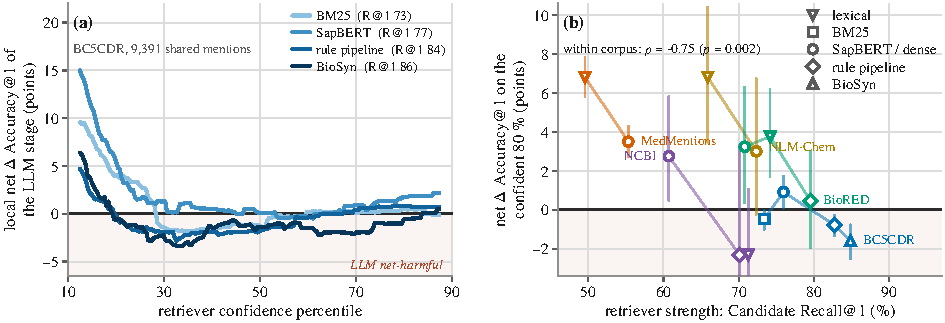
\includegraphics[width=\textwidth]{fig1_value.pdf}
\caption{\textbf{The LLM stage pays off where the retriever is unsure, and turns
net-harmful in the middle once the retriever is strong.}
\textbf{(a)} Local net $\Delta$ Accuracy@1 of the LLM stage ($\text{P4}-\text{P3}$)
in a sliding window covering $25\%$ of each run, over the percentile of the
retriever's own top1$-$top2 score gap. Colour is that run's Candidate Recall@1, so
the ordering of the curves \emph{is} retriever strength; a rank axis is used
because the score scales differ across retrievers. All eight runs use the same
zero-shot Qwen3-4B disambiguator. Every curve is strongly positive at low
confidence; only the strong-retriever curves cross into the shaded net-harmful
region, and they do so in the \emph{middle} of the confidence range, not at the
top.
\textbf{(b)} The same effect as one number per run: net $\Delta$ Accuracy@1 on the
$80\%$ of mentions the retriever is most confident about, against Candidate
Recall@1, with document-level bootstrap $95\%$ CIs and an OLS fit
(slope $-0.17$ points per point of Recall@1, $r=-0.82$, $p=0.013$; Spearman
$\rho=-0.90$, $p=0.002$; zero crossing at Recall@1 $\approx 80$). Beyond that
point the LLM stage is a net cost on everything except the mentions the retriever
is least sure about.}
\label{fig:value}
\end{figure*}

\begin{figure*}[t]\centering
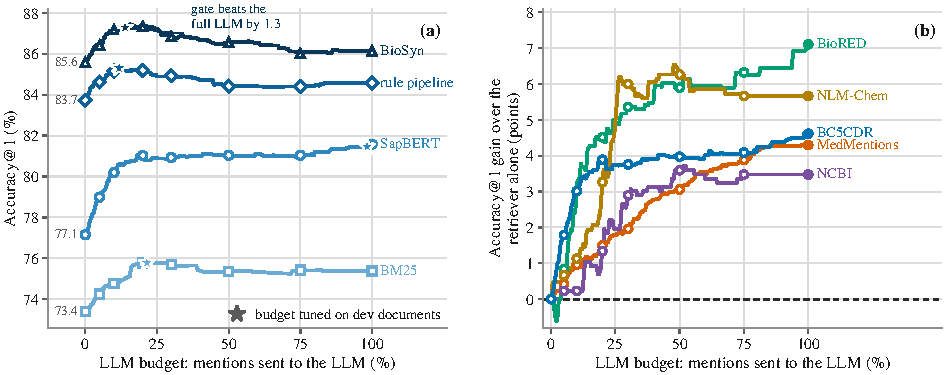
\includegraphics[width=\textwidth]{fig2_budget.pdf}
\caption{\textbf{Accuracy@1 against the LLM budget.} The gate routes the
least-confident mentions first, so budget $b$ means ``call the LLM on the $b\%$ of
mentions with the smallest top1$-$top2 gap''; $b=0$ is the retriever alone and
$b=100$ is the LLM on everything. $\bigstar$ marks the budget chosen on half the
\emph{documents} and evaluated on the other half.
\textbf{(a)} BC5CDR, four retrievers on the $9{,}391$ mentions all four cover.
As the retriever strengthens the curve turns over: BM25 and SapBERT are
monotone, whereas the rule pipeline and BioSyn peak at $12$--$14\%$ of the calls
and then decline, ending $0.7$ and $1.3$ points \emph{below} their own optimum.
\textbf{(b)} Gain over the retriever alone for one dense-retrieval run per
dataset; the same shape holds across corpora, with the weak-retriever datasets
(MedMentions, NCBI) still climbing at $100\%$.}
\label{fig:budget}
\end{figure*}
